\section{XMPT Tool Interface}
\label{section:xmpt}


\subsection{Overview}

XMPT is the tool interface of XMP and inspired by OMPT, which is the
tool interface of OpenMP \cite{ompt}.
%
Hence, XMPT is designed as event-based and callback-based as OMPT;
that is, for each event at runtime, the corresponding callback is
invoked. One or more XMPT events are defined correspondig to each of XMP
constructs and coarray-related actions (e.g. remote write/read and
synchronization).

XMPT is preliminarily implemented in the Omni XMP compiler \ref{chap2},
and used in MUST \cite{MUST-project} and experimentally in Extrae
\cite{Extrae-project}. More details of the application of XMPT in MUST 
is described in \label{chapter:mspmd-chapter}.


\subsection{Specification}

\subsubsection{Initialization}

Tool developers can provide the \|xmpt_initialize| function in which
they register a callback for each of the XMPT events of their interset,
as follows.

{\small
\begin{Cexample}
void xmpt_initialize(...){
 xmpt_set_callback(xmpt_event_bcast_begin, callback_bcast_begin);
 xmpt_set_callback(xmpt_event_bcast_end, callback_bcast_end);
 ...
}
\end{Cexample}
}

\sloppy
In the above example, the tool developer implements callbacks\\
\|callback_bcast_begin| and \|callback_bcast_end| that interact with
his/her tool.
\fussy

When an XMP program starts execution, the XMP runtime implicitly invokes
\|xmpt_initialize|, if provided, to set up the callbacks.

\subsubsection{Events}

XMPT defines XMPT events each of which corresponds to an XMP
construct or a coarray-related action. Below is the list of XMPT
events. For each of the events, the function signature of the
corresponding callback is specifically defined. Note that the ones from
\|xmpt_event_coarray_remote_write| to\\ \|xmpt_event_sync_images_end|
are coarray-related.

\begin{verbatim}
xmpt_event_task_begin
xmpt_event_task_end
xmpt_event_tasks_begin
xmpt_event_tasks_end
xmpt_event_loop_begin
xmpt_event_loop_end
xmpt_event_array_begin
xmpt_event_array_end
xmpt_event_reflect_begin
xmpt_event_reflect_begin_async
xmpt_event_reflect_end
xmpt_event_gmove_begin
xmpt_event_gmove_begin_async
xmpt_event_gmove_end
xmpt_event_barrier_begin
xmpt_event_barrier_end
xmpt_event_reduction_begin
xmpt_event_reduction_begin_async
xmpt_event_reduction_end
xmpt_event_bcast_begin
xmpt_event_bcast_begin_async
xmpt_event_bcast_end
xmpt_event_wait_async_begin
xmpt_event_wait_async_end
xmpt_event_coarray_remote_write
xmpt_event_coarray_remote_read 
xmpt_event_coarray_local_write
xmpt_event_coarray_local_read
xmpt_event_sync_memory_begin
xmpt_event_sync_memory_end
xmpt_event_sync_all_begin
xmpt_event_sync_all_end
xmpt_event_sync_image_begin
xmpt_event_sync_image_end
xmpt_event_sync_images_all_begin
xmpt_event_sync_images_all_end
xmpt_event_sync_images_begin
xmpt_event_sync_images_end
\end{verbatim}

\sloppy
When one of the XMPT events for which callbacks are registered occurs at
runtime, the corresponding callback is invoked by the XMP runtime. For
example, if callbacks are registered for events
\|xmpt_event_bcast_begin| and\\ \|xmpt_event_bcast_end| as in the example
in the previous section, tha callbacks \|callback_bcast_begin| and
\|callback_bcast_end| are invoked immediately before and after each of
\|bcast| constructs, respectively.
\fussy

The XMP runtime passes therein all the information about the construct,
including the mapping of the target global arrays, to the
callback as its parameters. Thus, the tool is able to extract necessary
information from the arguments.

% Procedure calls in XMP are almost the same as those in the base language.
% %
% Procedure calls between other languages or to external libraries
% are also allowed if the base language supports them. 

% In the below example, a function/subroutine \|sub1()| calls another
% function/subroutine \|sub2()| with a {\darray} \|x| as an
% argument.

% \begin{XCexample}
% void sub1(){
% #pragma xmp nodes p[2]
% #pragma xmp template t[10]
% #pragma xmp distribute t[block] onto p
%   double x[10];
% #pragma xmp align x[i] with t[i]
%   sub2(x);
% }

% void sub2(double a[10]){
% #pragma xmp nodes p[2]
% #pragma xmp template t[10]
% #pragma xmp distribute t[block] onto p
%   double a[10];
% #pragma xmp align a[i] with t[i]
%   :
% }
% \end{XCexample}

% \begin{XFexample}
% subroutine sub1()
% !$xmp nodes p(2)
% !$xmp template t(10)
% !$xmp distribute t(block) onto p
%   real x(10)
% !$xmp align x(i) with t(i)
%   call sub2(x)
% end subroutine

% subroutine sub2(a)
% !$xmp nodes p(2)
% !$xmp template t(10)
% !$xmp distribute t(block) onto p
%   real a(10)
% !$xmp align a(i) with t(i)
%   :
% end subroutine
% \end{XFexample}

% % If the programmer wants to use distributed arrays in arguments as distributed arrays
% % in the called procedure,
% % %
% % you need to redefine the shape of the distributed array in the procedure.

% To handle a parameter or dummy argument as a {\bf global data} in the
% callee procedure, the programmer need to explicitly distribute it with
% an \|align| directive.

% \begin{figure}
%   \centering
%   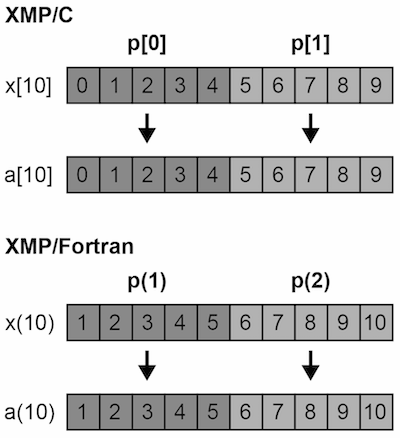
\includegraphics{figs/destributed_array.png}
%   \caption{Passing a global argument to a global parameter.}
% \end{figure}

% % However, if the programmer wants to use the distributed array in the argument as a
% % replicated array in the called procedure, you do not need to redefine
% % them.

% If no \|align| directive is specified in the callee procedure for a
% parameter or dummy argument that is declared as a {\bf global data} in the
% caller procedure, it is handled as if it were declared in the callee
% procedure as a {\bf local data} on each {\node}, as follows.

% \begin{XCexample}
% void sub1(){
% #pragma xmp nodes p[2]
% #pragma xmp template t[10]
% #pragma xmp distribute t[block] onto p
%   double x[10];
% #pragma xmp align x[i] with t[i]
%   sub2(x);
% }

% void sub2(double a[5]){
%   :
% }
% \end{XCexample}

% \begin{XFexample}
% subroutine sub1()
% !$xmp nodes p(2)
% !$xmp template t(10)
% !$xmp distribute t(block) onto p
%   real x(10)
% !$xmp align x(i) with t(i)
%   call sub2(x)
% end subroutine

% subroutine sub2(a)
%   real a(5)
%   :
% end subroutine
% \end{XFexample}

% \begin{figure}
%   \centering
%   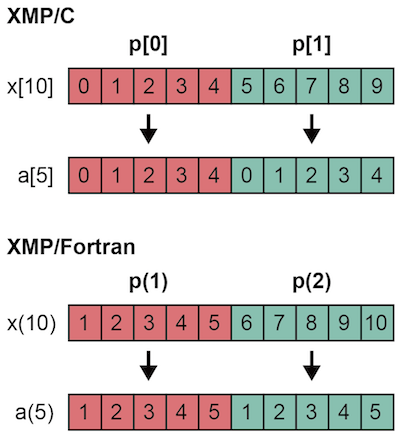
\includegraphics{figs/duplicated_array.png}
%   \caption{Passing a global argument to a local parameter.}
% \end{figure}